\section{Introduction}
\subsection{Software}
\begin{definition}[Software]
    Software besteht aus verschiedenen Komponenten und Artefakten, darunter:
    \begin{itemize}
        \item Das ausführbare Programm und die dazugehörigen Daten
        \item Konfigurationsdateien zur Anpassung und Steuerung des Systems
        \item Systemdokumentation, einschließlich Architekturmodelle, Entwurfsdokumente und technische Spezifikationen
        \item Benutzerdokumentation, wie Handbücker und Anleitungen
        \item Unterstützungsressourcen, etwa Updates, Benutzerforen und Support-Tools
    \end{itemize}
\end{definition}
\subsubsection{Arten von Software}
\begin{enumerate}
    \item \fatsf{Anwendungssoftware}
    \begin{itemize}
        \item Wird direkt vom Nutzer verwendet
        \item Umfasst allgemeine Programme (z.B. Textverarbeitung) und spezialisierte Software (z.B. CAD, IDE)
    \end{itemize}
    \item \fatsf{Systemsoftware}
    \begin{itemize}
        \item Ermöglicht den Betrieb des Computers, ohne direkte Interaktion mit dem Nutzer
        \item \fatsf{Betriebssysteme (OS):} Verwalten Hardware-Ressourcen und bieten eine Plattform für Anwendungen (z.B. Windows, macOS, Linux)
        \item \fatsf{Gerätetreiber:} Erlauben die Kommunikation zwischen OS und Hardware
        \item \fatsf{Dienstprograme:} Unterstützten Wartung und Optimierung (z.B. Defragmentierung, Backup)
        \item \fatsf{BIOS/Firmware:} Steuert grundlegende Hardware-Funktionen vor dem Laden des OS
    \end{itemize}
    \item \fatsf{Software as a Service (SaaS):} 
    \begin{itemize}
        \item Läuft in der Cloud und wird über das Internet genutzt
        \item Vorteile: Keine lokale Installation, automatische Updates, skalierbar und flexibel
        \item Beispiele: Microsoft 265, Google Workspace, Salesforce, Slack
        \item Herausforderungen: Abhängigkeit vom Internet, Datenschutzrisiken, begrenzte Anpassbarkeit
    \end{itemize}
\end{enumerate}
\subsection{Engineering}
\begin{definition}[Engineering]
    Anwendung wissenschaftlicher Prinzipien zur Konstruktion von Maschinen, Bauwerken und Systemen mit klar definierten Prozessen und Phasen:
    \begin{enumerate}
        \item \fatsf{Analyse} (Zweck, Belastungen)
        \item \fatsf{Design} (Pläne, CAD-Modelle)
        \item \fatsf{Evaluation} (Simulation, Berechnungen)
        \item \fatsf{Konstruktion} (überwacht, kontrolliert)
        \item \fatsf{Qualitätsprüfung} (z.B. TÜV)
    \end{enumerate}
\end{definition}
\subsubsection{Besonderheiten des Software Engineerings}
\begin{itemize}
    \item \fatsf{Software = Information} $\rightarrow$ Unabhängig von Speichermedium oder Transportweg, einfach zu kopieren und verteilen
    \item \fatsf{Ubiquitäre Konnektivität} $\rightarrow$ Ständiger Internetzugriff durch mobile Kommunikation ermöglicht neue Anwendungen
    \item \fatsf{Konsequenzen:}
    \begin{itemize}
        \item Keine klaren physischen Grenzen zwischen Subsystemen
        \item Geringe Verteilungskosten $\rightarrow$ Updates schnell, aber kurze Lebenszyklen
        \item Eingeschränkte Kontrolle über Updates $\rightarrow$ Veraltete Versionen bleiben im Umlauf (z.B. 13\% der Android-Geräte mit Version $\leq$ 9.x)
        \item Fehler breiten sich schnell aus $\rightarrow$ Hohe Innovationsgeschwindigkeit, aber große Angriffsfläche für Sicherheitsprobleme
    \end{itemize}
\end{itemize}
\subsection{Further Software Characteristics}
\begin{itemize}
    \item Software does not wear out, \red{but its environment does}
    \begin{itemize}
        \item Subject to continuous \red{change} in hardware, need to adapt
        \item Support for \red{new requirements}, use cases, etc.
    \end{itemize}
    \begin{infoBox}
        Auch wenn Software selbst nicht \enquote{altert}, ist sie kontinuierlichen Veränderungen in ihrer Umgebung ausgesetzt, um relevant, kompatibel und sicher zu bleiben, muss sie sich diesen Änderungen anpassen
    \end{infoBox}
    \item Software \red{lifetime} often much longer than expected
    \begin{infoBox}
        Software wird häufig länger genutzt, als ursprünglich vorgesehen. Entwickler planen typischerweise eine bestimmte Nutzungsdauer oder erwarten, dass die Software nach einigen Jahren durch neuere Versionen oder andere Produkte ersetzt wird. In der Praxis bleibt Software jedoch oft weit über diesen Zeitraum hinaus im Einsatz, sei es, weil sie gut funktioniert, weil die Nutzer keine Notwendigkeit für ein Upgrade sehen oder weil der Ersatz teuer oder kompliziert ist.
    \end{infoBox}
    \begin{itemize}
        \item Next to impossible to anticipate \red{unknown requirements}
    \end{itemize}
     \begin{infoBox}
         Wenn Software entwickelt wird, kennen die Entwickler die aktuellen Anforderungen und Anwendungsfälle, die die Software unterstützen soll. Was jedoch schwer vorhersehbar ist, sind zukünftige Anforderungen, die erst entstehen, wenn sich die Technologie oder die Bedürfnisse der Nutzer ändern. Neue gesetzliche Anforderungen, Sicherheitsbedrohungen, Änderungen in der Hardware oder neue Benutzeranforderungen tauchen oft unerwartet auf und können zusätzliche Funktionen, Anpassungen oder Änderungen an der Software erforderlich machen.
     \end{infoBox}
     \item Some software properties are hard to \red{measure}
     \begin{infoBox}
         Software besitzt verschiedene Eigenschaften, die nicht so einfach quantifiziert oder bewertet werden können. Während bestimmte Aspekte wie die Anzahl der Fehler oder die Geschwindigkeit einer Software objektiv messbar sind, gibt es andere Eigenschaften, die schwerer greifbar sind, z. B. die Qualität, der Fortschritt bei der Entwicklung oder die Widerstandsfähigkeit (Resilienz) gegenüber Problemen.
     \end{infoBox}
     \begin{itemize}
         \item How do lines of code relate to software \red{quality}?
         \begin{infoBox}
             Die Anzahl der Zeilen Code (Lines of Code, LOC) ist eine oft verwendete Metrik in der Softwareentwicklung, aber sie sagt wenig über die tatsächliche Qualität der Software aus. Mehr Code bedeutet nicht unbedingt bessere Software – es könnte sogar das Gegenteil der Fall sein, weil längerer Code schwerer zu warten und potenziell fehleranfälliger ist. Es kommt mehr darauf an, wie der Code strukturiert ist, ob er gut lesbar und modular ist und ob er Best Practices folgt. Ein kürzerer, gut geschriebener Code kann also von höherer Qualität sein als ein langer, unstrukturierter Code.
         \end{infoBox}
         \item How do we measure \red{progress}?
         \begin{infoBox}
             Den Fortschritt bei der Softwareentwicklung zu messen, ist ebenfalls eine Herausforderung. Traditionelle Metriken wie „Anzahl abgeschlossener Aufgaben“ oder „Zeilen Code“ geben keine Auskunft darüber, ob die Software tatsächlich bereit für den Einsatz ist oder die gewünschte Qualität erreicht hat. Der Fortschritt hängt von verschiedenen Faktoren ab, darunter der Umsetzung neuer Funktionen, der Behebung von Fehlern und der Verbesserung der Benutzerfreundlichkeit. Oft werden agile Methoden verwendet, bei denen der Fortschritt anhand von erledigten „User Stories“ oder „Sprints“ gemessen wird, aber auch diese Metriken haben ihre Grenzen.
         \end{infoBox}
         \item How to measure \red{resilience}?
         \begin{infoBox}
             Resilienz bezeichnet die Fähigkeit einer Software, auf Probleme oder Störungen robust zu reagieren, also beispielsweise nach einem Fehler weiter zu funktionieren oder schnell wiederhergestellt zu werden. Es ist schwierig, diese Eigenschaft direkt zu messen, weil sie sich oft erst in realen Szenarien zeigt, wenn unerwartete Ereignisse eintreten. Tests wie „Chaos Engineering“ versuchen, Resilienz durch das absichtliche Einführen von Fehlern oder Ausfällen zu messen, um zu prüfen, wie gut die Software darauf reagiert.
         \end{infoBox}
     \end{itemize}
\end{itemize}
\red{Need to adapt notion of engineering to specific software characteristics}
\begin{infoBox}
    Das Ingenieurwesen muss an die besonderen Eigenschaften von Software angepasst werden, um deren immateriellen Charakter, die ständigen Veränderungen, die komplexen Interaktionen und die schwer messbaren Eigenschaften angemessen zu berücksichtigen
\end{infoBox}
\subsection{Modified View on Software Engineering}
\begin{defBox}[title=Software Engineering (IEEE Standards Board\, Glossary of SE TErminology)]
    \begin{enumerate}
        \item The application of a systematic disciplined quantifiable approach to the development, \red{operation}, and \red{maintenance} of software; that is, the application of engineering to software
        \begin{infoBox}
            Diese Definition beschreibt Software Engineering als einen Ansatz, der methodisch und strukturiert ist, ähnlich wie in anderen Ingenieurdisziplinen. Die Kernaspekte sind:
            \begin{itemize}
                \item \fatsf{Systematisch:} Es wird ein geplanter und strukturierter Ansatz verfolgt, um Software zu entwickeln. Das bedeutet, dass die Schritte im Entwicklungsprozess klar definiert und organisiert sind, um ein vorhersehbares und kontrollierbares Ergebnis zu erreichen.
                \item \fatsf{Diszipliniert:} Es gibt feste Praktiken, Regeln und Verfahren, die befolgt werden, um sicherzustellen, dass die Software den Anforderungen entspricht. Disziplin bedeutet in diesem Kontext, dass Standards und Best Practices eingehalten werden, um Fehler zu minimieren und eine hohe Qualität zu gewährleisten.
                \item \fatsf{Quantifizierbar:} Es wird versucht, verschiedene Aspekte des Softwareprozesses messbar zu machen. Dazu gehören z. B. die Produktivität, die Anzahl der Fehler, die Zeit bis zur Fertigstellung oder die Leistung der Software. Diese Messbarkeit hilft dabei, den Fortschritt und die Qualität besser zu überwachen und Entscheidungen datenbasiert zu treffen.
                \item \fatsf{Entwicklung, Betrieb und Wartung:} Software Engineering umfasst nicht nur die Entwicklung neuer Software, sondern auch den Betrieb (wie die Software eingesetzt wird) und die Wartung (das Beheben von Fehlern, Durchführen von Updates oder Anpassungen an veränderte Anforderungen).
            \end{itemize}
            Kurz gesagt: Software Engineering wendet Prinzipien des Ingenieurwesens auf Software an, um den gesamten Lebenszyklus von Softwareprojekten systematisch und effektiv zu gestalten.
        \end{infoBox}
        \item The study of approaches in (1)
        \begin{infoBox}
            Dieser zweite Teil der Definition besagt, dass Software Engineering auch die wissenschaftliche Untersuchung und das Studium der verschiedenen Methoden, Techniken und Prinzipien umfasst, die im ersten Punkt beschrieben wurden. Es geht darum, herauszufinden, welche Ansätze und Praktiken am effektivsten sind, um qualitativ hochwertige Software zu entwickeln, zu betreiben und zu warten.
        \end{infoBox}
    \end{enumerate}
\end{defBox}
Definition fails to include (but others do): \red{Mathematical an scientific principles}
\subsection{What? vs How?}
\begin{minipage}{0.5\textwidth}
    \centering
    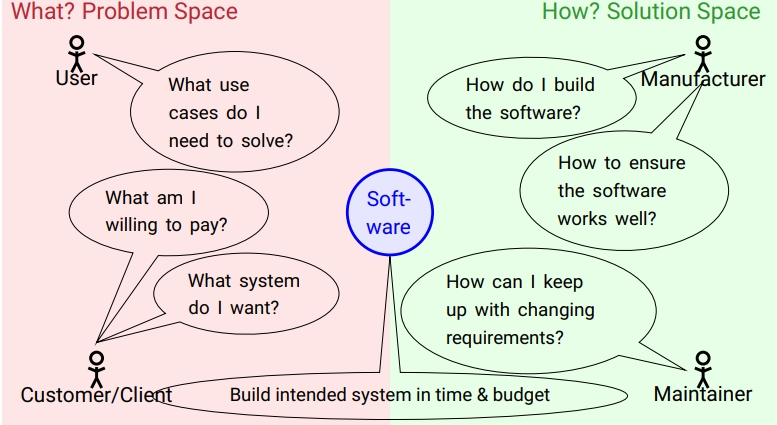
\includegraphics[width=1\textwidth]{Images/What vs How.jpeg}
\end{minipage}
\begin{minipage}{0.5\textwidth}
    \centering
    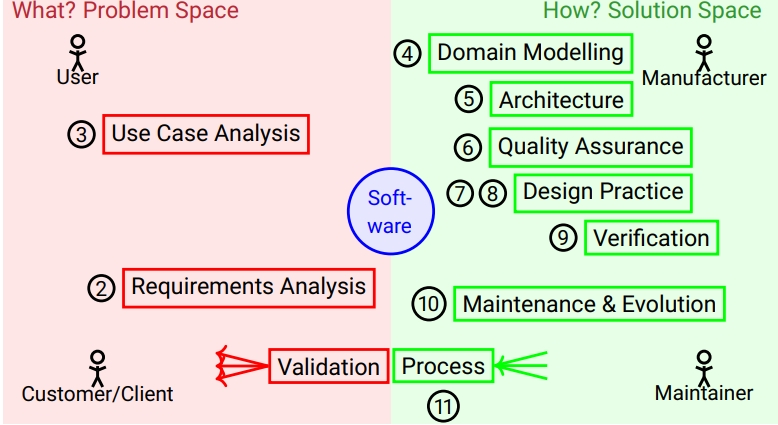
\includegraphics[width=1\textwidth]{Images/What vs How 2.jpeg}
\end{minipage}
\subsection{Software Engineering: Demarcation Lines}
\begin{infoBox}[title=Was ist Systems Engineering?]
    Systems Engineering beschäftigt sich mit der Planung, Entwicklung und Umsetzung von komplexen Systemen, die aus verschiedenen Komponenten bestehen, wie Hardware, Software, Mensch-Maschine-Schnittstellen und Betriebsprozessen. Das Ziel ist es, ein Gesamtsystem zu entwerfen, das den Anforderungen entspricht und gut funktioniert. Systems Engineering bezieht sich also auf das „große Ganze“ und umfasst alle Schritte von der Konzeptionsphase bis zur Implementierung und Wartung des Systems.
\end{infoBox}
\begin{infoBox}[title=Was ist Software Engineering?]
    Software Engineering hingegen konzentriert sich speziell auf die Entwicklung, den Betrieb und die Wartung von Software. Es ist ein Teilbereich des Systems Engineering, wenn das Gesamtsystem Software enthält oder auf Software basiert. Das Ziel ist es, Software systematisch und diszipliniert zu entwickeln, um sie zuverlässig und qualitativ hochwertig zu machen.
\end{infoBox}
\begin{defBox}[title=Systems Engineering (Systemtechnik) vs. Software Engineering]
    \begin{itemize}
        \item \red{Overall systemic} objectives and requirements
        \begin{infoBox}
            \begin{itemize}
                \item Beim Systems Engineering werden zunächste die Gesamtziele und Anforderungen des gesamten Systems definiert. Dazu gehört, festzulegen, was das System insgesamt leisten soll, welche Leistungsmerkmale es haben muss und welche Einschränkungen zu berücksichtigen sind
                \item Software Engineering fokussiert sich dann darauf, diese Anforderungen für den Softwaretiel des Systems umzusetzen
            \end{itemize}
        \end{infoBox}
        \item Assigning system functions between \red{hardware and software}
        \begin{infoBox}
            \begin{itemize}
                \item Systems Engineering befasst sich mitder Entscheidung, welche Funktionen durch Hardware und welche durch Software realisiert werden sollen. Diese Entscheidung beeinflusst die Gesamtarchitektur des Systems
                \item Software Engineering setzt diese Entscheidungen um, indem es die Software entwickelt, die die zugewiesenen Funktionen übernimmt
            \end{itemize}
        \end{infoBox}
        \item Defining interfaces between \red{hardware and software}
        \begin{infoBox}
            \begin{itemize}
                \item Systems Engineering legt die Schnittstellen zwischen den verschiedenen Systemkomponenten fest, z.B. wie Hardware und Software miteinander kommunizieren sollen
                \item Software Engineering implementiert dann diese Schnittstellen auf der Softwareseite, um sicherzustellen, dass die Software korrekt mit der Hardware interagiert
            \end{itemize}
        \end{infoBox}
        \item Full \red{system acceptance} tests
        \begin{infoBox}
            \begin{itemize}
                \item Systems Engineering umfasst umfassende Tests des gesamten Systems, um sicherzustellen, dass alle Komponenten (Hardware, Software, Mensch-Maschine-Schnittstellen usw.) nahtlos zusammenarbeiten und die definierten Anforderungen erfüllen
                \item Software Engineering führt dagegen spezifische Tests für die Software durch, um deren Funktionalität, Leistung und Qualität sicherzustellen, bevor sie in die Systemtests einfließt
            \end{itemize}
        \end{infoBox}
    \end{itemize}
    are aspects of \red{Systems Engineering}: Software Engineering is a \blue{part of} Systems Engineering (where systems are \red{software systems})
\end{defBox}
\begin{defBox}[title=Computer Science vs. Software Engineering]
    Software Engineering ist a subfield of Computer Science (at least in Europe)
\end{defBox}
\subsection{Importance of Software Production Environment}
\begin{defBox}
    Social aspects of Software Engineering: important, but beyont this course
\end{defBox}
\begin{defBox}[title=Software Development Problems caused by Environment]
    \begin{itemize}
        \item Lack of customer/user involvement:
        \begin{itemize}
            \item insufficient validation
            \item inadequate specification: incomplete, ambiguous, inconsistent
        \end{itemize}
        \item Constantly \red{changing requirements} (moving target)
        \begin{itemize}
            \item gets worse the longer it takes to ship the product
            \item (erroneous) perception: changing software is easier than hardware
        \end{itemize}
        \item Insufficient \red{training} of software engineers
        \item \red{Management} (until recently, almost no Comuper Scientists)
        \item \red{Unsuitable} (prescribed) methods, languages, tools
    \end{itemize}
\end{defBox}
\begin{infoBox}
    Die Softwareentwicklung wird stark von der Umgebung beeinflusst, in der sie stattfindet. Mangelnde Kundenbeteiligung, ständig wechselnde Anforderungen, unzureichende Schulung der Entwickler, mangelndes technisches Management und ungeeignete Methoden oder Werkzeuge können alle zu ernsthaften Problemen führen. Es ist wichtig, diese Herausforderungen zu erkennen und proaktive Maßnahmen zu ergreifen, um sicherzustellen, dass die Softwareentwicklung erfolgreich verläuft und die gewünschten Ergebnisse erzielt werden.
\end{infoBox}
\begin{defBox}[title=Detection an Error Presumes an Expectation (Requirement)]
    \begin{infoBox}
        Die Idee hier ist, dass man einen Fehler nur erkennen kann, wenn man eine Vorstellung davon hat, was korrekt oder erwatungsgemäß sein sollte. Diese Vorstellung wird durch die Anforderungen definiert
        \begin{itemize}
            \item \fatsf{Anforderungen als Maßstab:} Anforderungen dienen als Maßstab für das , was die Software tun sollte. Wenn ein Programm funktioniert, wie es soll, und die Erwartungen erfüllt, gehen wir davon aus, dass es keine Fehler gibt
        \end{itemize}
    \end{infoBox}
    \begin{itemize}
        \item Few errors are \enquote{obvious} (such as a crash)
        \begin{infoBox}
            \begin{itemize}
                \item \fatsf{Offensichtliche Fehler:} Einige Fehler sind sofort erkennbar, wie ein Programm, das abstürzt. Solche Fehler sind leicht zu identifizieren und zu beheben, weil sie sofortige Auswirkungen auf die Benutzer haben
                \item \fatsf{Stille Fehler:} Viele Fehler sind jedoch nicht sofort offensichtlich und können lange unentdeckt bleiben. Zum Beispiel:
                \begin{itemize}
                    \item \fatsf{Falsches Ergebnis einer komplexen Berechnung:} Wenn ein Programm falsche Ergebnisse liefert, ohne dass es abstürzt oder eine Fehlermeldung ausgibt, kann es lange dauern, bis dieser Fehler erkannt wird
                \end{itemize}
            \end{itemize}
        \end{infoBox}
        \item Without precise \red{requirements} threre are no \red{errors}:\\
        INABIAF - \enquote{It´s not a bug, it´s a feature}
        \begin{infoBox}
            Wenn die Anforderungen unklar, unvollständig oder mehrdeutig sind, ist es schwierig, einen Fehler zu definieren. In solchen Fällen kann eine Abweichung von einer ungenauen Anforderung nicht wirklich als Fehler betrachtet werden, da es nicht klar ist, was die Software leisten sollte.
            \begin{itemize}
                \item \fatsf{INABIAF:} Das Akronym steht für \enquote{It´s Not a Bug, It´s a Feature} und beschreibt die Haltung, dass eine unerwartete Verhaltensweise als gewollte Funktion angesehen werden kann, wenn die Anforderungen nicht klar definiert sind. Dies kaann zu Verwirrung und Frustration bei Benutzern führen 
            \end{itemize}
        \end{infoBox}
        \item Many errors traceable to \blue{VVD}: \red{Validation, Verifikation, Documentation}
    \end{itemize}
    $\Rightarrow$ \blue{Insufficient match between requirements and realization}
\end{defBox}
\begin{defBox}
    Error in design/code $\subsetneq$ Software \red{construction} error 
\end{defBox}
\begin{defBox}[title=\enquote{Software} Errors present in every Construction Phase]
    \begin{itemize}
        \item Requirements analysis:
        \begin{itemize}
            \item Unanticipated requirements
            \item Silently changed requirements
        \end{itemize}
        \item Use case analysis
        \item Domain modelling      \item Verification 
        \item Design                \item Validation 
        \item Algorithms            \item Documentation
        \item Coding                \item Maintenance
    \end{itemize}
\end{defBox}
\subsection{Take-home Message:}
\begin{defBox}
    Software development must be economical
\end{defBox}
\begin{defBox}
    Software development must be safe and ensure high quality
\end{defBox}
\begin{defBox}
    Software development must follow scientific \& engineering principles
\end{defBox}
